\documentclass[]{cxs-software}
\usepackage{graphicx}
\usepackage{hyperref}
\usepackage{eurosym}
\usepackage{pifont}
%\usepackage{tocloft}
\usepackage{amsmath}
\usepackage{subfigure}
\usepackage{fancyhdr}
\usepackage{fancyvrb}
\usepackage{booktabs}
\usepackage{comment}
\usepackage{import}
\usepackage{listings}
\usepackage{tikz}
\usepackage{html}
%\begin{htmlonly}
%  \usepackage{verbatim}
%  \providecommand{\lstlisting}[2][]{\verbatim{#2}}
%  \renewcommand*{\lstlisting}{\verbatim}
%\end{htmlonly}
\lstnewenvironment{myverbatim}{}{}

\RequirePackage[dvips]{color}

\definecolor{mycolour}{rgb}{0.05,0.2,0.5}
\definecolor{gray}{rgb}{0.9,0.9,0.9}
\definecolor{darkgray}{rgb}{0.3,0.3,0.3}

%\usepackage{doxygen}
\pagestyle{fancy}

\lstset{
language=C++,
basicstyle=\ttfamily\color{mycolour},                  % Code font, Examples: \footnotesize, \ttfamily
commentstyle=\color{darkgray},            % Comments font
backgroundcolor=\color{gray},
basewidth=0.5em,
breaklines=true,
}   

\usetikzlibrary{shapes.arrows,chains,positioning}

%\usepackage{color,fancyvrb}
%\renewcommand\FancyVerbFormatLine[1]
%{\colorbox{gray}{\makebox[\linewidth][l]{#1}}}

%\DefineShortVerb{\!}

%\makeatletter
%\renewcommand*\l@section{\bf{\color{mycolour}\sffamily{#1}}}
%\renewcommand*\l@subsection{\bf{\color{mycolour}\sffamily{#1}}}
%\renewcommand*\l@subsubsection{\bf{\color{mycolour}\sffamily{#1}}}
%\makeatother

%\makeatletter
%\newcommand{\mysection}[1]{%
%  \section*{\bf{\color{mycolour}\sffamily{#1}}}}
%\newcommand{\mysubsection}[1]{%
%  \subsection*{\bf{\color{mycolour}\sffamily{#1}}}}
%\newcommand{\mysubsubsection}[1]{%
%  \subsubsection*{\color{mycolour}\sffamily{#1}}}
%\makeatother

\begin{document}
\sffamily

\vspace{6cm}

\maketitle

\setcounter{tocdepth}{3}
%\tableofcontents\pdfbookmark[0]{Table of Contents}{toc}
\tableofcontents

\newpage


%\section{Introduction}

%The high resolution imaging of finite nano-scale objects has been
%shown to be possible due to .........
%the developement of Coherent Diffractive
%Imaging (CDI) techniques~\cite{}.

%Wavelength limited resolution...

%lense-less X-ray imaging techniques have proved to
%be a promising technique for imaging nano-scale biological objects.

%The phase information is recovered computationally, through use of
%iterative algorithms~\cite{}. 

%The rapid developement in theory and experimentation in this field has
%created a need for common software tools within the CDI community.
%HAWKE~\cite{}, a plane-wave CDI reconstruction package, was was
%developed for this purpose. The need for Fresnel coherent diffractive
%imag



%In this paper we describe a computer program 

%.which provide a user
%friendly, reliable and fast method for reconstructing X-ray
%diffraction data.


%The program extends upon this existing software, by providing:
%\begin{itemize}
%\item A full choice of iterative algorithms, including customised
%  algorithms. In~\cite{} it was demonstrated that all reconstruction
%  algorithms could be expressed through X combinations of projection
%  operators. ......
%\item Fresnel Coherent Diffractive Imaging algorithms~\cite{} have
%  been implemented.
%\item Ptychographic~\cite{} and Phase-Diverse~\cite{} CDI have also
%  been implemented.
%\end{itemize}


%The software consists of a C++ library, interface to IDL, command-line
%tools in addition to example code and documentation. 

%......

%- motivation
%- review of similar software
%- goals and users


\section{Overview}

In the development of experimental infrastructure, software is an
important element which is often overlooked. For X-ray Coherent
Diffractive Imaging (CDI), in particular, computational inversion of
the measured diffraction intensity is an integral part of the image
reconstruction process. The proliferation of phase retrieval
algorithms has created the need for common software tools which
encompass all these approaches. The DIXE (Diffractive Imaging for
X-rays and Electrons) software package aims to provide a set of phase
retrieval tools which are robust, efficient and available to the wider
CDI community.

In this documentation, we introduce the software package, DIXE (also
known as cxs-software), which is able to reconstruct and simulate
X-ray diffraction data for plane-wave, Fresnel, ptychographic and
phase-diverse CDI. To the best of our knowledge, this is the first
standard software package which includes all of these different
approaches. The software allows for any choice of iterative algorithm,
including customized algorithms, and also includes the 'shrinkwrap'
algorithm. For Fresnel CDI, additional complex constraints on the
transmission function may also be used. The software consists of a C++
library, binding to IDL and command-line tools, in addition to example
code and documentation. It has been tested on the Mac, Windows and
Ubuntu operating systems. It is issued under the GNU public license.

It is assumed that readers of this manual are familiar with the
relevant literature describing the CDI algorithms implemented in DIXE,
we will therefore not repeat this information here. Please refer to
any of the review~\cite{} for more information on this topic. We
intend that this manual is used in the following way:
\begin{itemize}
\item New users should follow the instructions provided for
  installation, Section \ref{installation}, followed by ``Getting
  Started'', Section \ref{getting started}.
\item The remainder of the manual is provided as a reference for users
  who are already using the code. Section \ref{how to}, ``How to'', gives
  instructions on how to complete specific tasks and control the CDI
  reconstruction. The appendices document the important routines,
  functions and classes provided by the \name library.
\end{itemize}
This version of the software is a developement version and we welcome
feedback on any aspect of the software package: functionality,
installation, documentation etc. Please email ..... for questions or
comments.

\section{Installation Instructions}
\label{installation}

The software is available for download from the software website as either,
\begin{itemize}
\item a tar ball containing the software source code or
\item a pre-compiled Windows 32 bit binary file.
\end{itemize}

For Windows users who only wish to use the IDL capabilities or
command-line tools we recommend downloading the Windows binary file. For
all other users, we recommend downloading the source code package.

\subsection{Installing from Source Code}

\subsubsection{Linux}

Currently the code depends on a few other libraries which will need to
be installed prior to installing this package:
\begin{itemize}
\item g++\cite{} - for compilation of C++ source code (we have tested with version 4.4.3)
\item fftw\cite{} - for fast Fourier transforms.
\item libtiff\cite{} - for reading and writing to tiff files.
\item HDF libraries\cite{} - for reading (and not yet writing to) hdf4
  files. Note that this one depends on a few other libraries, so make
  sure there's are also installed.
\end{itemize}

Ubuntu users can easily install the extra packages using the synaptic
package manager. Look for libfftw3-dev, libtiff4-dev and libhdf4-dev.

Download our source code from the website and put
it into an appropriate directory. Unzip and untar the source code: 
\begin{myverbatim}
  gunzip CXS.rel_0.4.tar.gz 
  tar -xvvf CXS.rel_0.4.tar
\end{myverbatim}

Now change to the directory cxs\_software and compile the source code: 
\begin{myverbatim}
  cd cxs_software 
  ./configure 
  make
\end{myverbatim}

If ./configure doesn't finish by making a set of "Makefiles", the
dependent libraries probably haven't been installed correctly or
./configure does not know their location.

The result of compiling (if successful) are libraries and header files
(in the /lib and /include directories) and some example programs which
are ready to execute.

The Makefile in examples/ shows how the libraries can be linked to
your own code and 

The source files in the examples/ directory e.g. real\_example.c
demonstrate how the libraries can be used withing a user's own
code. The Makefile in examples/ shows how a user's code can be
compiled and the \name libraries linked.

\subsubsection{Mac}

\begin{enumerate}
\item Install Xcode\cite{}. This is a big download and you first have to register as a developer. Once installed, this is a nice text editor too.
\item Install fink\cite{}. Following the instructions exactly as it says. You
  use fink like {\tt apt get} on linux to install the fftw and hdf
  packages. Make sure you select the correct releases of these.
\item Get and build the fftw, libtiff and hdf packages using fink
\item Download the \name source code from the website
\item Follow the install instruction for linux, except, replace ./configure with 
\begin{myverbatim}
  ./configure --with-fftw_inc=/sw/include --with-fftw_lib=/sw/lib CXX="g++ -arch i386" --with-mfhdf_inc=/sw/include --enable-checking
\end{myverbatim}
The ``--with'' flags will tell the compiler where to look for the
external packages.  The CXX="g++ -arch i386" relates to your
computer's architecture. This is for a late 2010 macbook pro running
10.6, try this, if it doesn't work, try looking up the relevant
information for your computer. --enable-checking is just in case.
\item Type make, as in the linux instructions.
\end{enumerate}

\subsubsection{Windows with Cygwin}

Cygwin\cite{} provides a linux/unix type environment for Windows (the
interface is basically a unix style terminal). Installing the CXS
source code in this environment is very similar to installing it in
linux/unix and (in my opinion) makes modifying and recompiling the
code a bit easier than it would be in Windows otherwise. First you
will need to install cygwin. You can do this by going to
http://www.cygwin.com/, scrolling to the bottom of the page and
clicking on "Install or update now\ (using setup.exe)". Open setup.exe
and follow the installation instructions. Apart from the "Package
Selection" screen, used the default options. When you get to the
"Package Selection" screen leave "All" on "Default" and add the
additional packages by searching for them and then clicking on them:
\begin{itemize}
\item libhdf5-devel - These are libraries for reading hdf files.
\item gcc4-g++ - This is the c/c++ compiler I like to use.
\item make - This is used to automatically compile the package.
\item xemacs or emacs - This is a text/code editor
\item libfftw3-devel - This is a fast Fourier transform library.
\item libtiff-devel - This is a library for reading/writing tiff image files.
\item sunrpc
\item libjpeg-devel
\item zlib-devel
\end{itemize}

Note that you can update the packages which are installed after you've
installed cygwin just by clicking on setup.exe again (it remembers
which are installed). If you get an error during the post-installation
phase (error code 128) it maybe due to a virus checkers interfering
with the cygwin installation.

Install the HDF4 libraries. There is no package for this in the
package manager so go to http://www.hdfgroup.org/release4/obtain.html
and download their cygwin binary. Unzip the file using the standard
windows tool and extract it into your home cygwin directory (which
should be something like
C:\textbackslash{}cygwin\textbackslash{}home\textbackslash{}your\_user\_name). The directory
hdf4.2.5-cygwin-szip should be made. The HDF library also needs the
szip library to work correctly. Download this from \\
http://www.hdfgroup.org/ftp/lib-external/szip/2.0/bin/cygwin/szip\_cygwin\_encoder.zip  \\
and also extract it into your home directory on cygwin.

Next, download the cxs software here and put it into your home
directory on cygwin (C:\textbackslash{}cygwin\textbackslash{}home\textbackslash{}your\_user\_name). Open cygwin and
unzip and untar the package:
\begin{myverbatim}
$ gunzip CXS.rel_0.4.tar.gz 
$ tar -xvvf CXS.rel_0.4.tar 
\end{myverbatim}

When you type ls you should see the directory "cxs\_software" plus a
few others. Change into the cxs\_software directory:
\begin{myverbatim}
$ cd cxs_software 
\end{myverbatim}
Tell the package where your hdf and szip libraries files are located
(replace the "user\_name" with your cygwin user name):
\begin{myverbatim}
$ ./configure --with-mfhdf_lib=/home/"user_name"/hdf4.2.5-cygwin-szip/lib --with-mfhdf_inc=/home/"user_name"/hdf4.2.5-cygwin-szip/include --with-sz_lib=/home/"user_name"/szip_cygwin_encoder/lib 
\end{myverbatim}

If you get an errror, check that the paths given to configure are
correct; the lib directories should have files starting with "lib" and
the include directory should have files ending in ".h". If configure
worked correctly, then compile the libraries and examples:
\begin{myverbatim}
$ make
\end{myverbatim}

Hopefully you won't get any errors and when you look in the lib/ and
include/ directories you will see some files. The libraries can be
useful if you ever need to create your own code (similar to the
examples). The examples show how the libraries can be used. 

\begin{comment}
--------------------------------------
Change into the example directory:
\begin{myverbatim}
$ cd examples 
\end{myverbatim}
and run one of the examples. e.g.: 
\begin{myverbatim}
$ ./PlanarCDI_example.exe
\end{myverbatim}

If everything is working correcting, you should see some text output
(counting the iterations). If you look at this directory in the
Windows browser you should see that some .ppm image files are created
which give you the reconstruction image for various number of iterations.

Have a look at the code in more detail to see what's going on: 
\begin{myverbatim}
$ xemacs PlanarCDI_example.c 
\end{myverbatim}
and edit some variables to see what happens (eg. change the reconstruction algorithm). 
Then recompile and rerun the example: 
\begin{myverbatim}
$ make 
$ ./PlanarCDI_example.exe
\end{myverbatim}
-------------------------
\end{comment}

\subsection{Installing from the Windows Binary}

Download the package (binary file) from the main webpage. Executing
the .msi file should automatically start the installation. Select
which directory you want the files to be installed in (if it's not
you're own machine you probably won't have permission to install into
``Program Files''). Once installed you can start using the library and
command line executable files. Look at the README file which comes
with the distribution to find out more. 

To uninstall, go to "Control Panel", go to "Add/Remove program", find
CXSSoftware and remove it.


\section{Getting Started}
\label{getting started}

\subsection{For Users on Osiris}

Note: this section is only applicable to users who are members of
the ARC Centre of Excellence in Coherent X-ray Science (CXS).

If you are not familiar with linux or c and want to quickly use the
software without the hassle of installing many packages, the simplest
way is by logging into OSIRIS and using it there. This will also be
useful to know how to do in the long run because the computing power
available there is more than your laptop/desktop. The first step is to
ask for an account on OSIRIS if you don't already have one (and are a
member of CXS). Then follow the steps below for logging in, and for
setting up and running the software.

\subsubsection{Logging into Osiris from a Linux/Unix/Mac Machine}

Open a terminal and type: 
\begin{myverbatim}
  ssh -X11 -2 osiris.ph.unimelb.edu.au 
\end{myverbatim}
The "-X11 -2" enables you to view graphics on osiris.

\subsubsection{Logging into Osiris from Windows}

On Windows, you will need to install an ssh client. Most people
(including me) recommend the program putty for this.  After you
install it, test it works by logging into osiris:
\begin{enumerate}
\item Open putty 
\item In the host name field type "@osiris.ph.unimelb.edu.au" 
\item Make sure the connection type is set to "ssh" 
\item Save these setting by typing in a saved session name. e.g
  "osiris" and clicking on "Save". Next time to open putty to can load
  these setting by clicking on "osiris" and then "Load".
\item Now click on "Open". A terminal should open with a prompt asking
  for you password. After you enter it correctly you are logged into
  osiris.
\item End your session by typing "exit"
\end{enumerate}

You are now half way there. You can log in, but you won't be able to
view any images which are stored on osiris yet. To be able to do this,
you need to install an X-windows server (graphical information can be
passed back to your computer once you have this). I found Xming to be
good. I installed it with the default options ("normal Putty").

I also found that I need to install Xming-fonts in order for the
"emacs" text editor to disply fonts correctly. During the set-up I
ticked all the boxes so that all the fonts were installed.

Now, each time you want to log into osiris you will need to run Xming
first. It will run in the background, so all you'll see when it's
running is a small icon on the tool bar. You can close it once you've
finished with your putty session.

Finally go into putty again, and load your "osiris" session. 
\begin{enumerate}
\item Configure it for X windows by clicking on "SSH" under "Connection" in the tree on the left hand side of the screen. 
\item click on "X11" 
\item On the right hand side of the screen click on "Enable X11 forwarding". 
\item Click on "session" in the left-hand tree. 
\item And save these settings. 
\item You are now ready to test it out. Click on "Open" and log in. type "emacs test" and you hopefully a window will pop up. Don't worry too much about what this is for now. Close the window and you are ready to start.
\end{enumerate}

\subsubsection{Setting up your environment on Osiris}
\label{osiris-setup}
Once you have successfully logged in, append your PATH variable to the
directory where the cxs programs are located. This can be done by
typing:
\begin{myverbatim}
  export PATH=$PATH:/data/nadia/cxs_software_rel_0.4/cxs_software/bin 
\end{myverbatim}

You now have available all of the command line tools listed here. Note
that this will only work for your current session on osiris. To make
it permanent, open the file ".bash\_profile" in your home area:
\begin{myverbatim}
  emacs .bash_profile 
\end{myverbatim}
Add the line above to the end of the file, save and then close it (use
the menu or type "xs" followed by "xc" while holding down the Ctrl
key).

If you plan to work with IDL you will also need to update your
LD\_LIBRARY\_PATH with the wrapper library path:
\begin{myverbatim}
  export LD_LIBRARY_PATH=$LD_LIBRARY_PATH:/data/nadia/cxs_software_dev/cxs_software/interfaces/idl/ 
\end{myverbatim}
and update the IDL\_PATH with the IDL module location:
\begin{myverbatim}
  export IDL_PATH="${IDL_PATH}:\:/data/nadia/cxs_software_dev/cxs_software/interfaces/idl/"
\end{myverbatim}

\subsubsection{Running the Commandline Tool}

The simplest way to run reconstruction is to use the
CDI\_reconstruction.exe command line tool. It takes three arguements as
input:
\begin{itemize}
\item a configuration file, 
\item the reconstruction type: planar, fresnel\_wf or fresnel and
\item a seed for the initial random estimate. 
\end{itemize}
If you don't give the seed value, "0" is used as the default, and if
you don't give the reconstuction type, "planar" is assumed.

Test out the program by running it with one of the example
configuration files: 
\begin{myverbatim}
   ./CDI_reconstruction.exe planar_example.config
\end{myverbatim}
You should see output telling you the iteration number and the
error. The error is a measure of the difference between the
diffraction data and the reconstructed diffraction (the usual chi
squared given in the literature). You can kill the process at any time
by typing Ctrl-C or you can wait for it to finish if you like.

Now look into the configuration file by typing: 
\begin{myverbatim}
   emacs planar_example.config 
\end{myverbatim}
You can see that the data and support file names are given. Type: 
\begin{myverbatim}
   gthumb image_files/planar_support.tiff 
\end{myverbatim}
to view the support. The data file can't be viewed with gthumb because
it's in binary format, however you can convert it to a !.ppm! file using
one of the other command line tools and then view it: 
\begin{myverbatim}
   dbin2ppm.exe image_files/planar_data.dbin planar_data.ppm 1024 1024 
   gthumb planar_data.ppm
\end{myverbatim}

The CDI\_reconstruction.exe program outputs a .ppm file of the current
magnitude of the estimated exit surface wave every 40 iterations. Type
ls again to see a list of these files (they should look something like
planar\_x.ppm, where x is the iteration number). View them using
gthumb. The reconstruction is slowly converging. Note that it may not
completely converge as the number of iterations performed in this
example is a lot less than usually used. The exit surface wave of the
final iteration is saved as a complex binary file (with the file
extension .cplx). You can view the magnitude and phase of the wave, by
using the cplx2ppm.exe command, followed by the gthumb command. You
can also use this file as the starting point for another
reconstruction (see planar\_example.config for instructions).

Now, try editing the configuration file: 
\begin{myverbatim}
   emacs planar_example.config 
\end{myverbatim}
e.g. with a different combination of reconstuction algorithms, a
different output rate, support file or shrink-wrap parameters etc. and
see what happends.

A similar example exists for the Fresnel case. This can be run by
first reconstructing the white field using 3-plane propogation:
\begin{myverbatim}
   ./CDI_reconstruction.exe fresnel_example.config fresnel_wf 
\end{myverbatim}
Then reconstruct the sample: 
\begin{myverbatim}
   ./CDI_reconstruction.exe fresnel_example.config fresnel
\end{myverbatim}

\subsubsection{Using the C/C++ Library}

The command line tools are useful to get started quickly, but if you
want full flexibility with the code, it's best to learn a little bit
of "c" and examples are provided for this as well. The same
reconstruction as planar.config performs can be done using
PlanarCDI\_example.c. Compile this code using the Makefile: make Now
when you type ls you should see a filenamed PlanarCDI\_example.exe. Run
this.
\begin{myverbatim}
./PlanarCDI_example.exe 
\end{myverbatim}
You should find it gives almost exactly the same output as the
CDI\_reconstuction program did. Have a look at the source code: emacs
PlanarCDI\_example.c edit it and recompile using make to see what
happens. Similarly, have a look at and Frsnel example:
FresnelCDI\_WF\_example.c and FresnelCDI\_example.c, and a simulation of
the object from the planar example: PlanarCDI\_simulation\_example.c.

Later, if you write your own "c" code, it's easy to compile and link
it with the libraries using the "Makefile" from the examples
directory. Edit the "EXAMPLE\_SRC" variable in the Makefile with the
name of your ".c" file, then type "make" on the command line to
compile it.

\subsubsection{Using the Library in IDL}

Some IDL wrapper have been written for the C++ library. This is useful
for people who are more familiar with IDL than C. It will give greater
flexibility than the command line program but doesn't allow to you use
all the features of the C++ library.

Begin by copying the IDL examples to your working directory, 
\begin{myverbatim}
cp /data/nadia/cxs_software_dev/cxs_software/interfaces/idl/*_example.pro ./ 
\end{myverbatim}
and run them: 
\begin{myverbatim}
idl planar_example.pro
\end{myverbatim}

Look at the .pro files to see what they do. 


\subsection{After Installing from Source}

Open a terminal and follow the instruction given for ``Users on
Osiris'', from Section \ref{osiris-setup} onwards. Replace the path to
the software on osiris,
``/data/nadia/cxs\_software\_dev/cxs\_software/'' in the instructions,
with the path where you installed the software.

\subsection{After Installing from the Window's Binary}





\section{How Tos}
\label{how to}

In this section, we describe how a number of common tasks can be
achieved using the software. More detail of the functionality
available can be found in the doxygen documentation () and IDL routine
documentation (). In the rest of this section, each of these steps are
described in more detail.


%\UndefineShortVerb{\!}
\begin{figure}
  \centering
  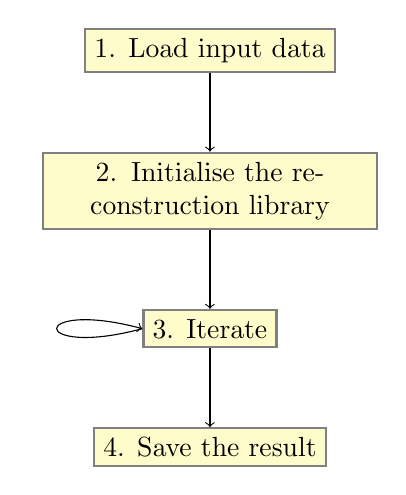
\begin{tikzpicture}[auto,mybox/.style={rectangle,draw=black!50,fill=yellow!20,thick},
      mybox2/.style={rectangle,draw=black!50,fill=blue!20,thick},
      mybox3/.style={rectangle,fill=black!10,minimum height=2cm,minimum width=5cm},
      mybox4/.style={rectangle,fill=white!10,minimum height=7.5cm,minimum width=7.5cm},
      mybox5/.style={rectangle}]
  
    \node[mybox] (load) {1. Load input data};
    \node[mybox] (initialise)   [below=of load,text width=4cm,text centered] {2. Initialise the reconstruction library};
    \node[mybox] (iterate)      [below=of initialise]    {3. Iterate};
    \node[mybox] (result)  [below=of iterate]    {4. Save the result};
              
    \draw [->] (load.south) -- (initialise.north);
    \draw [->] (initialise.south) -- (iterate.north);
    \draw [->] (iterate.west) to [->,loop left,looseness=16,min distance=15mm](iterate.west);
    \draw [->] (iterate.south) -- (result.north);              

  \end{tikzpicture}  
  \caption{\label{fig:reco}The basic steps involved in a CDI reconstruction}
\end{figure}

\begin{enumerate}

\item {\it Load input data} - Functions are provided for reading and writing
  to various image formats. More information is given in Section
  \ref{subsubsec:read_images}.
  
\item {\it Initialise the reconstruction library} - Whether you are
  performing plane-wave, Fresnel or Phase-diverse/Ptycographic
  reconstruction, you must initialise the library with a number of
  input: the diffraction and support data, initial estimate, and
  parameters which describe the experimental set-up. Please refer to
  Sections \ref{subsubsec:rec_planar,subsubsec:rec_fresnel,subsubsec:rec_phase_div}
  for specific instructions.
      
\item {\it Iterate} - At this stage the iterative algorithms developed by
  \cite[] are run. In the software library, an iteration can be
  performed simply by calling one function:
      
      {\bf In C++}
      \begin{myverbatim}[language=C++]
        planar.iterate();
      \end{myverbatim}
      
      {\bf In IDL}
      \begin{myverbatim}[language=IDL]
        ; Perform one iteration. The exit-
        ; surface-wave is return to 'result'  
        result = CXS_ITERATE()
        
        ; Perform 50 iterations
        result = CXS_ITERATE(50)
      \end{myverbatim}

      Various aspects of the reconstruction can be controlled, for
      example, the algorithm, the relaxation parameter and the
      shrinkwrap algorithm. How this can be achieve with the software
      is described in this section. 


    \item {\it Save the result} - Refer to Section \ref{subsubsec:write_images}.

\end{enumerate}



\begin{comment}    
  \begin{scope}[xshift=5.5cm,yshift=-2.5cm]
    
    \node [mybox4] (highlight){};
         
    %      \only<1>{
    \node [mybox2] (intensity) at (-1.5,-0.5) {scale intensity};
    \node [mybox2] (support) [right=of intensity] {apply support};
    
    \draw [->] (intensity.south) to [in=270,out=270] node [auto,swap] {propagate to sample plane}(support.south) ; 
    \draw [<-] (intensity.north) to [in=90,out=90] node [auto] {propagate to detector plane} (support.north) ;
    %      }
    

                  \uncover<2-5>{

                    \node [mybox4] {
                      
                      \begin{minipage}{6cm}
                        
                        \only<2>{
                          Functions are provided for reading hdf, tiff and ppm image
                          files. \\
                          
                          {\bf In C++} 
                          \begin{myverbatim}[language=C++]
                            //read in the data
                            Double_2D data;
                            read_image(``data_file_name.tiff'', data);
                            
                            //read in the support shape
                            Double_2D support;
                            read_image(``support_file_name.tiff'', support);
                          \end{myverbatim}
                          
                          {\bf In IDL}
                          \begin{myverbatim}[language=IDL]
                            data = CXS_READ_PPM(1024, 1024, 'data_file.ppm')
                          \end{myverbatim}
                          etc. or use one of IDLs built in libraries to get
                          the input in matrix form.
                        }
                        
                        \only<3>{
                          The reconstruction code must be initialised for either
                          plane-wave, Fresnel white-field, Fresnel or phase diverse
                          reconstruction. \\
                          
                          {\bf In C++} 
                          \begin{myverbatim}[language=C++]
                            //Create a complex 2D field which will
                            //hold the result of the reconstruction.
                            Complex_2D object_estimate(nx,ny);
                            
                            //Create the planar CDI object which will
                            //be used to perform the reconstruction.
                            PlanarCDI planar(object_estimate);
                            
                            //set the support and intensity
                            planar.set_support(support,false);
                            planar.set_intensity(data);
                          \end{myverbatim}
                              {\bf In IDL}
                              \begin{myverbatim}[language=IDL]
                                CXS_INIT_PLANAR, data, support
                              \end{myverbatim}
                        }
                          
\end{comment}

\DefineShortVerb{\!}


\subsection{Data Input/Output and Preparation}

\subsubsection{Read Image Files}

\label{subsec:read_images}

The software is capable of accepting data in hdf, tiff or ppm image
format. It can output as a grey scale tiff or ppm image with X bytes
per pixel. In addition data can be read and stored as a binary file of
doubles. This may be useful in situations where high prescision is
required. Similarly, two dimensional arrays of complex numbers, such
as those produced in the reconstruction, may be stored as a binary
file of fftw~\cite{} complex number types.

{\bf In C++} 
\begin{myverbatim}[language=C++]
  //read in the data
  Double_2D data;
  read_image(``data_file_name.tiff'', data);
  
  //read in the support shape
  Double_2D support;
  read_image(``support_file_name.tiff'', support);
  \end{myverbatim}

{\bf In IDL}
\begin{myverbatim}[language=IDL]
   data = CXS_READ_PPM(1024, 1024, 'data_file.ppm')
\end{myverbatim}
etc. or use one of IDLs built in libraries to get
the input in matrix form.


\subsubsection{Write Image Files}
\label{subsub:write_images}
Save the result to file.\\
                          
{\bf In C++} 
\begin{myverbatim}[language=C++]
  //write out the result:
  // - as a complex binary file
  write_cplx(temp_str.str(),object_estimate);
  // - just the magnitude as an image
  Double_2D object_mag;
  object_estimate.get_2d(MAG,object_mag);
  write_image("mag.tiff",object_mag);
\end{myverbatim}
                          
{\bf In IDL}
\begin{myverbatim}[language=IDL]
  ; Record the complex field to a binary file
  CXS_WRITE_CPLX, result, 'result_file.cplx'
\end{myverbatim}
The magnitude and phase of the complex matrix
can be viewed and saved using the standard IDL
routines.


%\subsubsection{Plot the average intensity versus frame number, full-frame and ROI}
%\subsubsection{Check for saturation/dead pixels}
%\subsubsection{Run correlations on data and white-fields}
%\subsubsection{Convert HDF files and extract header info}
\subsubsection{Convert between different file formats}



\subsubsection{Output Data on a Log Scale}

\subsubsection{Subtract the darkfield}
%\subsubsection{Check the beam stability in data over time}
%\subsubsection{Check correlations after dark-field subtraction}

\subsubsection{Merge (add or average) data files together}

\subsubsection{Determine the normalisation of the white-field to data}

\subsubsection{Get the autocorrelation function}


\subsection{Initialise a Reconstruction or Simulation}

\subsubsection{Perform plane-wave reconstruction}
\label{subsubsec:rec_planar}

\subsubsection{Perform Fresnel reconstruction}
\label{subsubsec:rec_fresnel}

\subsubsection{Perform Phase Diverse Reconstruction}
\label{subsubsec:rec_phase_div}



\subsection{Run and Steer a Reconstruction}


\subsubsection{Select the algorithm}

By default plane-wave CDI uses the ... algorithm and Fresnel CDI uses
the ... algorithm. This can be easily changed at any point in the
reconstruction using the method

\begin{myverbatim}
void PlanarCDI::set_algorithm(int alg) 	
\end{myverbatim}
Where the algorithm options are:
\begin{description} 
\item ER - error reduction 
\item BIO - basic input-output 
\item BOO - basic output-output 
\item HIO - hybrid input-output 
\item DM - difference map 
\item SF - solvent-flipping 
\item ASR - averaged successive reflections 
\item HPR - hybrid projection reflection 
\item RAAR - relaxed averaged alternating reflectors
\end{description}

For example, if you have an object of type FresnelCDI called ``fcdi'', and
you wish to change the algorithm to HIO:
\begin{myverbatim}
fcdi.set_algorithm(HIO) 	
\end{myverbatim}

In addition to this extensive list, custom algorithms can be
used. Iterative reconstruction algorithms can be expressed as a
combination of the following 5 operators: , , , and Where is the
support projection and is the intensity projection. These can be
combined to form a basis of 10 vectors (see Harray's review). The
parameters to this method set the coefficient for each of these
vectors. Note: the vector set is linearly dependant.

Please see page 22 of the H.M. Quiney review: TUTORIAL REVIEW,
Coherent diffractive imaging using short wavelength light sources,
Journal of Modern Optics, 2010, DOI: 10.1080/09500340.2010.495459

\begin{myverbatim}
void Planar::set_custom_algorithm (double m1,
double 	m2,
double 	m3,
double 	m4,
double 	m5,
double 	m6,
double 	m7,
double 	m8,
double 	m9,
double 	m10	 
)
\end{myverbatim}
			
Parameters:
m1 	Coefficient to the  term
m2 	Coefficient to the  term
m3 	Coefficient to the  term
m4 	Coefficient to the  term
m5 	Coefficient to the  term
m6 	Coefficient to the  term
m7 	Coefficient to the  term
m8 	Coefficient to the  term
m9 	Coefficient to the  term
m10 	Coefficient to the  term




In IDL, the routine ... can be called to select the algorithm.


\subsubsection{Update the support or use the shrink-wrap algorithm}

\subsubsection{How to stop a reconstuction, save the result and restart at the same place}

\subsubsection{How to modify the reconstruction algorithm by adding a new constraint}

\subsubsection{Refine the experimental parameters during reconstuction}


\subsection{Perform a Simulation}


\section{Performance}

Performance results for the software are given below for the speed at
which the code runs and for the amount of memory consumed. In
designing the code we have tried to find a good balance between
optimising the speed, reducing the memory used, and keeping the code
modulare and simple to read. There is always room to improve the
performance and we provide the figures below as a benchmark of the
current state of the software in version \ver.

\subsection{Speed}

\begin{table}
\begin{tabular}{lcc}
\toprule
   & Laptop & Cluster/Server \\
   & Iteration per Second & Iterations per Second \\
\midrule
PlanarCDI (ER) & 3.3  &  \\
PlanarCDI (HIO) & 2.7 & \\
FresnelCDI - white field 2.0 &   & \\
FresnelCDI & 2.7 & \\
FresnelCDI with Complex Constraints & 1.8 & \\
Phase-Diverse/Ptychography & & \\
\bottomrule
\end{tabular}

\caption{\label{table:speed} CPU time for a 1024$\times$1024 pixel reconstruction. Laptop - , Cluster - . The start-up time is a few seconds in each case. 
}

\end{table}



\subsection{Memory}

By default the fast fourier transform library used with \name is
single precision. We found no noticible lose in performance or
correctness by using single precision, however users may choose to use
double precision fast fourier transforms by adding the flag
``--enable-double-precision'' to ``./configure'' during installation.
The class Double\_2D, despite its name, will also use the same
precision as the fourier transform library and is single precision by
default.

\begin{table}[hbt!]
\begin{tabular}[hbt!]{lcc}
\toprule
&  Number of N$\times$N & With p=4, N=1024 \\
&  pixel arrays used & (MB) \\
\midrule
PlanarCDI (ER) & $4$ & 17 \\
PlanarCDI (HIO) & $10$ & 42  \\
FresnelCDI - white field & $4.5$ & 19 \\
FresnelCDI & $8.5$ & 36 \\
FresnelCDI with complex constraints & $11.5+c$ & 57 (c=2) \\
Phase-Diverse/Ptychography & $I(1+X) + 2M/N$ & 30,000 (I=400,M = 1100$^2$, \\
 &                 & X = FresnelCDI)  \\
\bottomrule
\end{tabular}

\caption{\label{table:memory}The memory used.......
In total the memory used will be the factor given in the second
coloumn of Figure \ref{table:memory} multiplied by $pN^2$.
(N - image side length in pixels, p - precision in bytes, 
c - number of complex constraint regions, I - number of images, 
M - area, in pixels, of the phase-diverse image,
X - number of arrays needed for a single reconstruction ) 
}
\end{table}





\appendix


\section{Class Description} 

\begin{figure}[htbp]
\centering
\includegraphics*[scale=0.3,viewport = 0 0 1500 1200]{cxs_class_diagram.eps}
\caption[]{The relationship between classes of the \name package.
\label{fig:class_diagram}}
\end{figure}



\section{IDL Routines}


\section{License}


\section{More Information}


\end{document}
